\documentclass{article}
\usepackage[utf8x]{inputenc}
\usepackage{ucs}
\usepackage{amsmath} 
\usepackage{amsfonts}
\usepackage{upgreek}
\usepackage[english,russian]{babel}
\usepackage{graphicx}
\usepackage{float}
\usepackage{textcomp}
\usepackage{hyperref}
\usepackage{geometry}
  \geometry{left=2cm}
  \geometry{right=1.5cm}
  \geometry{top=1cm}
  \geometry{bottom=2cm}
\usepackage{tikz}
\usepackage{ccaption}
\usepackage{multicol}
\setlength{\columnsep}{1.5cm}
\setlength{\columnseprule}{0.2pt}

\usepackage{listings}


\begin{document}
\pagestyle{plain}
\lstset{
  language=C,                % choose the language of the code
  basicstyle=\linespread{1.1}\ttfamily,
  columns=fixed,
  fontadjust=true,
  basewidth=0.5em,
  keywordstyle=\color{blue}\bfseries,
  commentstyle=\color{gray},
  stringstyle=\ttfamily\color{orange!50!black},
  showstringspaces=false,
  numbersep=5pt,
  numberstyle=\tiny\color{black},
  numberfirstline=true,
  stepnumber=1,                   % the step between two line-numbers.        
  numbersep=10pt,                  % how far the line-numbers are from the code
  backgroundcolor=\color{white},  % choose the background color. You must add \usepackage{color}
  showstringspaces=false,         % underline spaces within strings
  captionpos=b,                   % sets the caption-position to bottom
  breaklines=true,                % sets automatic line breaking
  breakatwhitespace=true,         % sets if automatic breaks should only happen at whitespace
  xleftmargin=.2in,
  extendedchars=\true,
  keepspaces = true,
}
\lstset{literate=%
   *{0}{{{\color{red!20!violet}0}}}1
    {1}{{{\color{red!20!violet}1}}}1
    {2}{{{\color{red!20!violet}2}}}1
    {3}{{{\color{red!20!violet}3}}}1
    {4}{{{\color{red!20!violet}4}}}1
    {5}{{{\color{red!20!violet}5}}}1
    {6}{{{\color{red!20!violet}6}}}1
    {7}{{{\color{red!20!violet}7}}}1
    {8}{{{\color{red!20!violet}8}}}1
    {9}{{{\color{red!20!violet}9}}}1
}

\title{Семинар \#8: Динамическое программирование. Классные задачи.\vspace{-5ex}}\date{}\maketitle
\section*{Задача о кузнечике:}
Кузнечик находится в начале координата (точке $x = 0$) и может прыгать вперёд на 1 шаг или на 2 шага. Найти \textit{количество разных путей} которыми кузнечик может добраться из точки $0$ до точки $x = n$. Пример одного из путей на рисунке:
\begin{center}
\includegraphics[scale=0.9]{../images/grasshopper.png}
\end{center}


\subsection*{Решение:}
Пусть $f(k)$ -- это количество всевозможных путей от точки $x = 0$ до точки $x = k$. Предположим, что мы знаем все $f(k)$ до $k = n - 1$. Как найти $f(n)$?\\
В точку $n$ кузнечик может попасть из точки $n - 1$ или из точки $n - 2$. Число возможных путей до точки $n$ равно сумме числа путей до точки $n - 1$ и числа путей до точки $n - 2$:
$$
f(n) = f(n-1) + f(n-2)
$$
Решение на языке C:
\begin{lstlisting}
#include <stdio.h>
#define MAX 100

int main()
{
	int f[MAX] = {};
	int n;
	scanf("%d", &n);
	f[0] = 1;
	f[1] = 1;

	for (int i = 2; i <= n; ++i)
	{
		f[i] = f[i-1] + f[i-2];
	}
	printf("%d\n", f[n]);
}
\end{lstlisting}

\subsection*{Задачи:}
\begin{itemize}
\item \textbf{СуперКузнечик:} Предположим, что кузнечик может прыгать на любое число шагов. Найдите \textit{количество разных путей} которыми кузнечик может добраться из точки $x = 0$ до точки $x = n$.

\item \textbf{Кузнечик на плоскости:} Кузнечик находится на плоскости в точке $(0, 0)$ и может прыгать на 1 шаг вправо или на 1 шаг вверх. Найдите \textit{количество разных путей} которыми кузнечик может добраться из точки $(0, 0)$ до точки $(n, m)$.
\begin{center}
\begin{tabular}{ c | c }
 вход & выход \\ \hline
 2 2 & 6  \\ 
 6 8 & 3003  \\ 
 10 10 & 184756  \\ 
\end{tabular}
\end{center}

\item \textbf{Кузнечик на платной дороге:} Пусть кузнечик может прыгать на 1, 2 или 3 шага на прямой. Но в каждой точке с кузнечика взимается плата -- некоторое целое число рублей. Плата в каждой точке задаётся в виде массива длины \texttt{n + 1} (от \texttt{0} до \texttt{n} включительно). Кузнечику нужно добраться из точки \texttt{x = 0} до точки \texttt{x = n}, заплатив как можно меньше. Найдите оптимальный путь кузнечика и количество рублей, которые должен он заплатить.\\
Например, для входа:
\begin{verbatim}
8
0 1 9 9 2 2 6 5 1
\end{verbatim}
Оптимальная плата и оптимальный путь будут равны:
\begin{verbatim}
6
0 1 4 5 8
\end{verbatim}
Протестируйте вашу программу на следующих тестах:
\begin{center}
\begin{tabular}{ c | c }
 вход & выход \\ \hline
 файл \texttt{grasshopper\_test\_0.txt} & \texttt{6}  \\
 										& \texttt{0 1 4 5 8}\\
 файл \texttt{grasshopper\_test\_1.txt} & \texttt{12}  \\
 										& \texttt{0 3 5 8 10}\\
 файл \texttt{grasshopper\_test\_2.txt} & \texttt{266}  \\
 										& \texttt{0 2 5 6 9 11 13 15 18 20 22 24 27 30 33 36 39 41 44 47 50}\\
 										& \texttt{53 56 59 62 64 66 69 72 75 78 80 82 85 87 90 92 95 98 100}\\
\end{tabular}
\end{center}
\end{itemize}

\section*{Задача о черепашке:}
Черепашка находится в вехнем левом углу прямоугольной таблицы. В каждой ячейке таблицы лежит определённое число кочанов капусты. Черепашка может двигаться либо вниз либо вправо по таблице на 1 шаг. Найдите такой путь, при котором черепашка съест наибольшее число кочанов капусты.
\begin{center}
\includegraphics[scale=0.8]{../images/turtle.png}
\end{center}
На вход задаче поступает файл с размером таблицы и самой таблицей. Нужно напечатать путь в виде строки из символов \texttt{R (Right)} и \texttt{D (Down)} и количество кочанов капусты на этом пути. Например, для таблицы на изображении программа должна выдать:
\begin{verbatim}
RRRDRDRRDR 58
\end{verbatim}
Протестируйте вашу программу на следующих тестах:
\begin{center}
\begin{tabular}{ c | c }
 вход & выход \\ \hline
 файл \texttt{turtle\_test\_0.txt} & \texttt{RRRDRDRRDR 58}  \\ 
 файл \texttt{turtle\_test\_1.txt} & \texttt{DRRRRRRRRRDDDDDDDD 244}  \\ 
 файл \texttt{turtle\_test\_2.txt} & \texttt{RRRRRRRRRRRDDRRDRRRRDDRDDDDRDRDDDRRDRRRRDDRRRDDDDDRDDRDDDRRRDRRRDDRRR}\\
                                   & \texttt{RRDRDDDDDRRDDRDRRRDDRRRDRRRRRRRRDDRRDRRDDDDDDDDDDDDDDRDDRDDDDDDDRRDRR}\\
                                   & \texttt{DDDDDRDRRRRDDRDDDDDRDDDDRRRRDRDDDRDRRDRDRDDRRRRRRRRDDDRRRDRD 2823}  \\ 
\end{tabular}
\end{center}

\section*{Подмассив максимальной суммы:}
Напишите программу, которая принимает на вход массив и находит непрерывный подмассив, имеющий наибольшую сумму. Например, для массива:
\begin{verbatim}
{5,   -4,   6, -9,   7,   4,  -9,  2,   4,  8, -7,  4,   3,  9,   5,  -4,  -3,  -3,  7,  -5}
\end{verbatim}
подмассив максимальной суммы будет такой:
\begin{verbatim}
{7,   4,  -9,  2,   4,  8, -7,  4,   3,  9,   5}
\end{verbatim}
\subsection*{Подсказка:}
$f(n)$ -- в этой задаче -- это сумма лучшего подмассива, который заканчивается в точке $n$. Также потребуется хранить $start(n)$ -- индекс первого элемента подмассива, который заканчивается в точке $n$.

\end{document}
